\begin{figure}
	\centering
	\begin{subfigure}{0.45\linewidth}
		\centering
		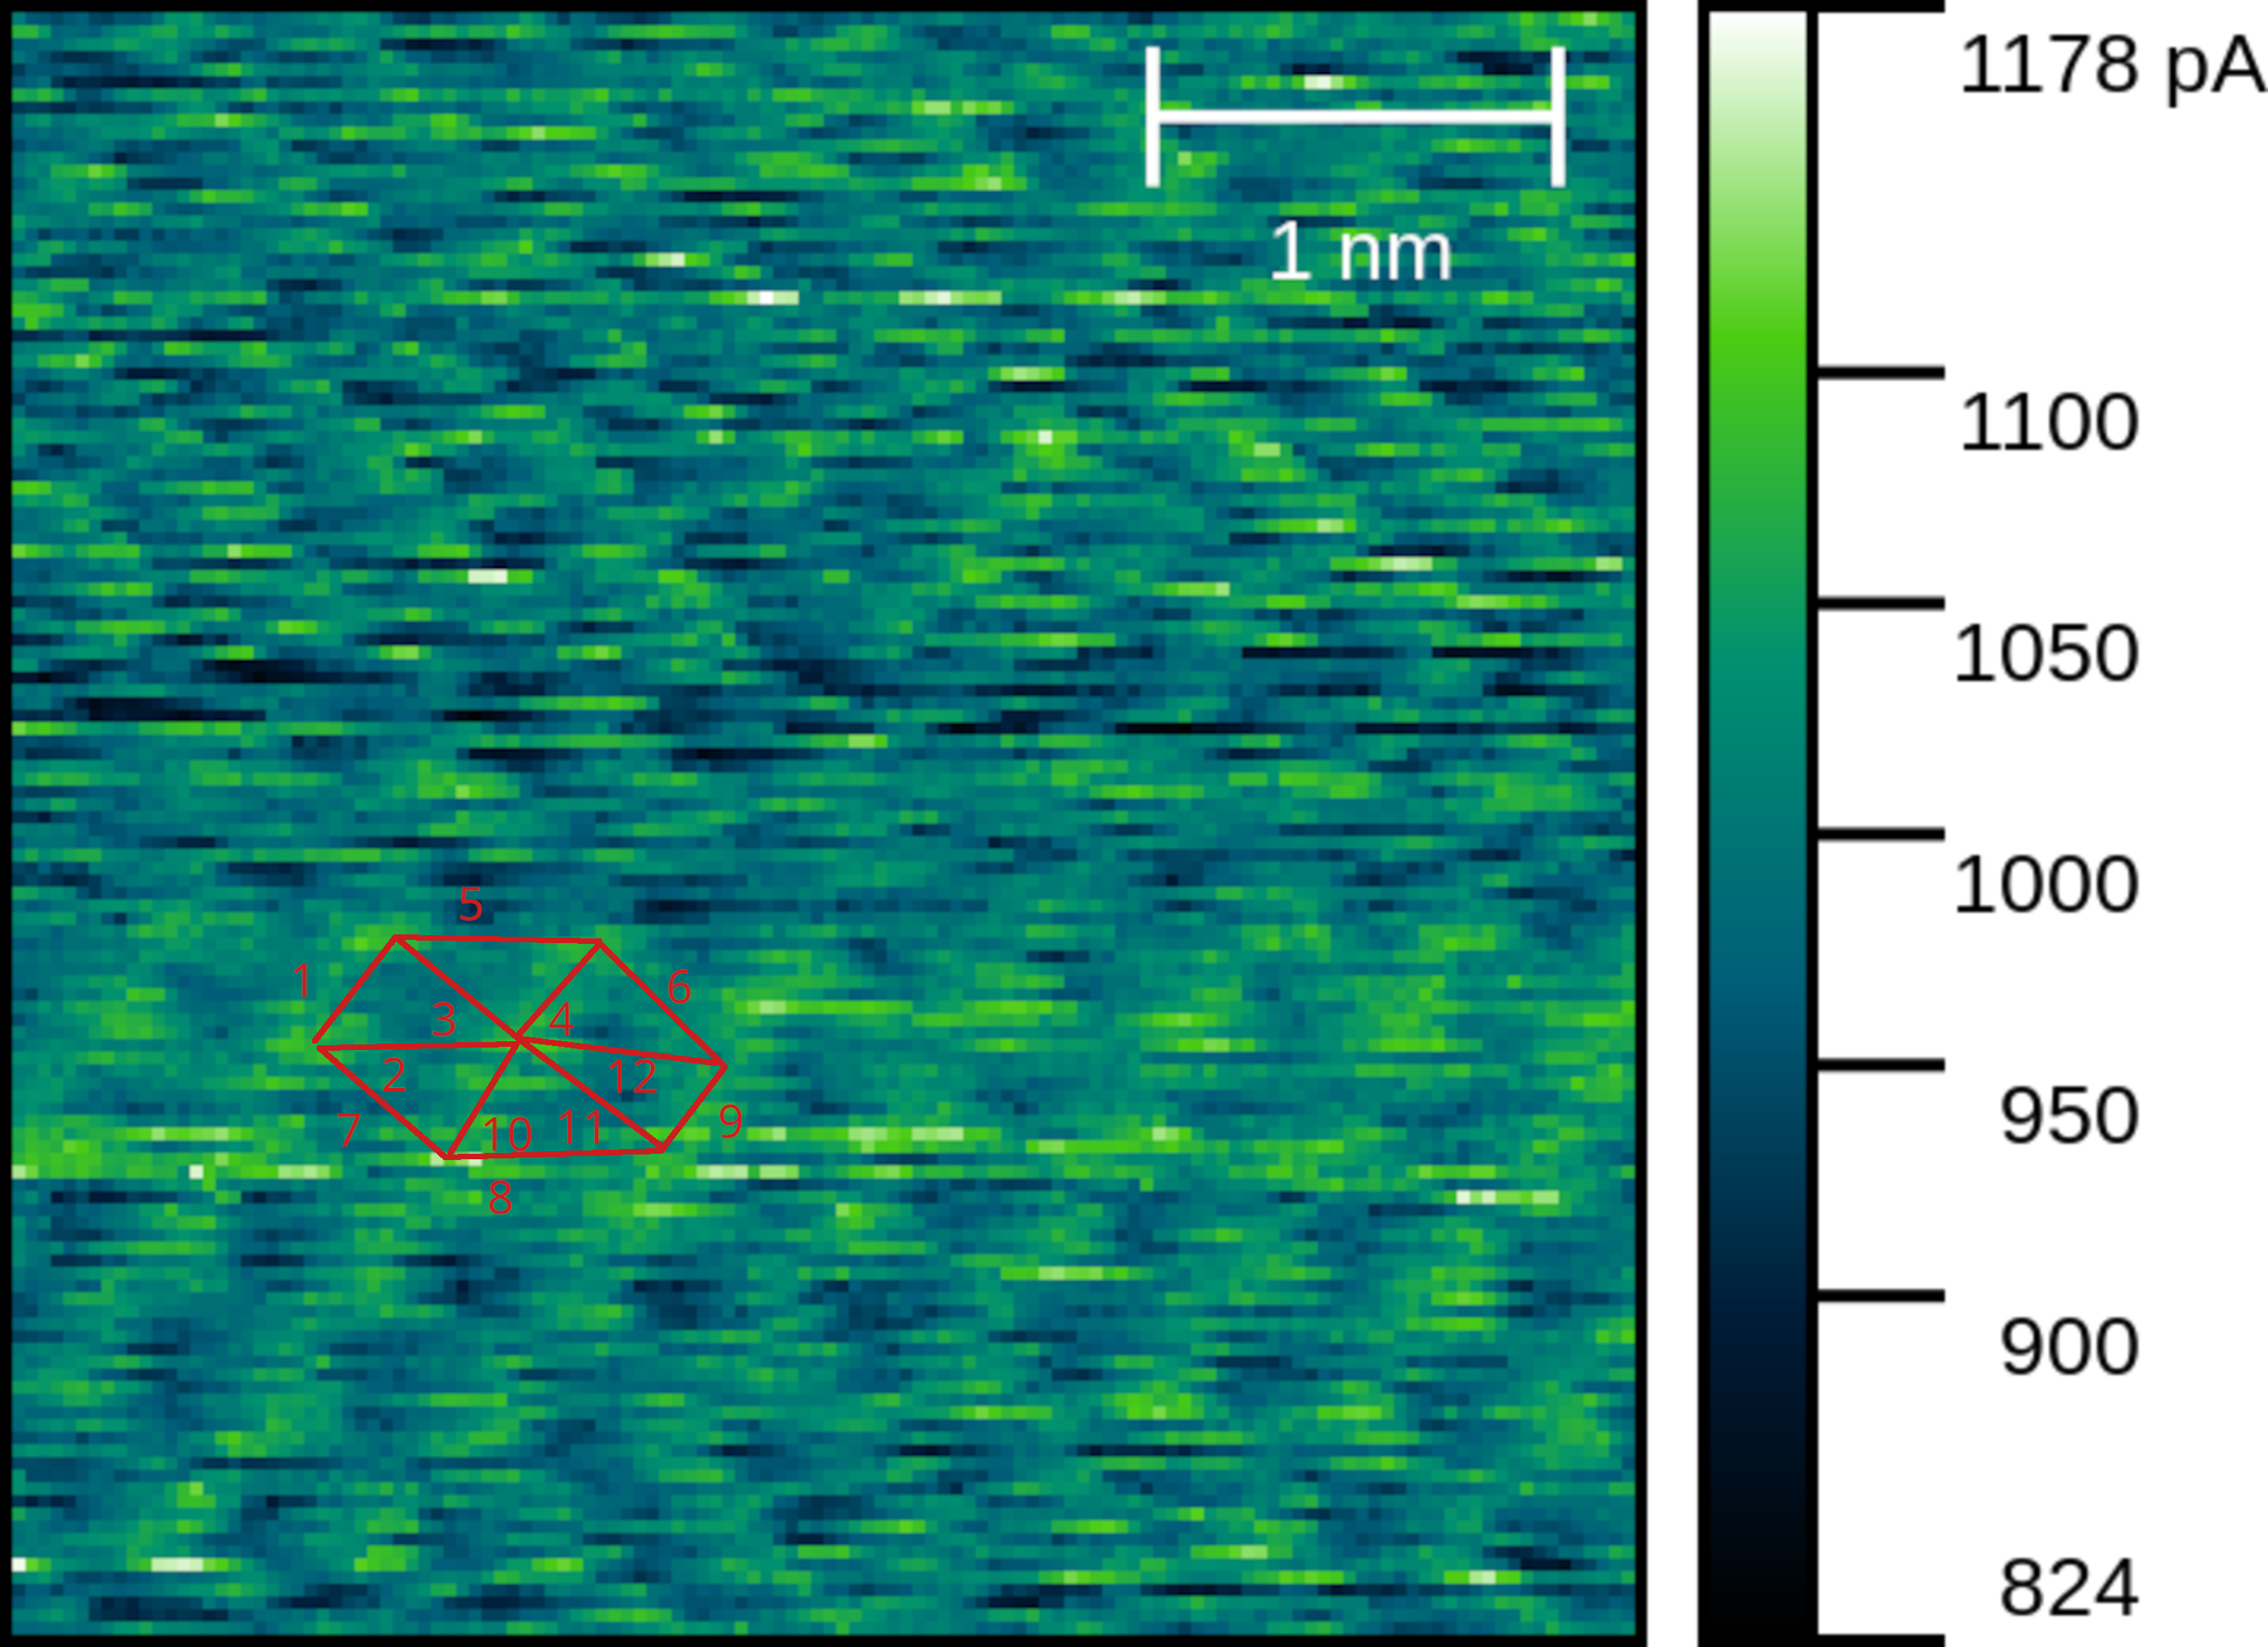
\includegraphics[width=\linewidth]{figs/HOPG10597_lines.png}
		\caption{Strommessung}
		\label{fig:hopg_rtm_4nm_1_cur}
	\end{subfigure}
	\hspace{.5cm}
	\begin{subfigure}{0.45\linewidth}
		\centering
		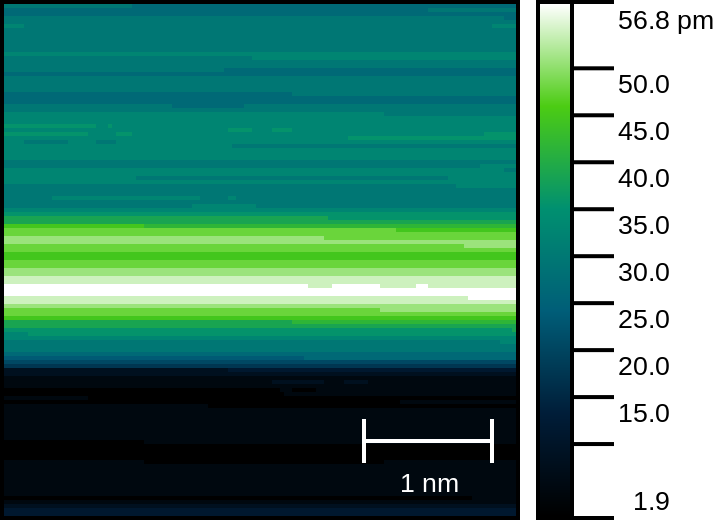
\includegraphics[width=\linewidth]{figs/HOPG10597_height.png}
		\caption{Abstandsmessung}
		\label{fig:hopg_rtm_4nm_1_height}
	\end{subfigure}
	\caption{RTM-Aufnahmen der HOPG-Probe. \textit{Image size} \SI{4}{\nano \meter},
	\textit{Rastergeschwindigkeit} \SI{77.5}{\nm\per \second}, \textit{Setpoint} \SI{1}{\nano \ampere},
	\textit{Tip voltage} \SI{0.1}{\volt}, \textit{P-Gain} \num{0}, \textit{I-Gain} \num{4},
	\textit{D-Gain} \num{0}, Spitze 2, \textit{Rotation} \SI{20}{\degree}.}
	\label{fig:hopg_rtm_1}
\end{figure}
